\documentclass[journal]{IEEEtran}
%\IEEEoverridecommandlockouts
% The preceding line is only needed to identify funding in the first footnote. If that is unneeded, please comment it out.

% listings package for code blocks
\usepackage{listings}
\usepackage{xcolor}
\usepackage{cite}
\usepackage{verbatim}
\usepackage{graphicx}
\usepackage{parskip}

\begin{document}

% overfull \hbox .. too wide 
\setlength{\emergencystretch}{12pt}
%\setlength{\parskip}{0pt} % 1ex plus 0.5ex minus 0.2ex}
\setlength{\parindent}{10pt}

\definecolor{codegreen}{rgb}{0,0.6,0}
\definecolor{codegray}{rgb}{0.5,0.5,0.5}
\definecolor{codepurple}{rgb}{0.58,0,0.82}
\definecolor{backcolour}{rgb}{0.95,0.95,0.92}

\lstdefinestyle{mystyle}{
    backgroundcolor=\color{backcolour},   
    commentstyle=\color{codegreen},
    keywordstyle=\color{magenta},
    numberstyle=\tiny\color{codegray},
    stringstyle=\color{codepurple},
    basicstyle=\ttfamily,
    breakatwhitespace=false,         
    breaklines=true,      
    postbreak=\mbox{\textcolor{red}{$\hookrightarrow$}\space},           
    captionpos=b,
}

\lstset{style=mystyle}

\title{Investigating Decision Trees}

\author{
\IEEEauthorblockN{Lillian Mueller}
\IEEEauthorblockA{lmuelle1@umd.edu}
\\
\IEEEauthorblockN{Regina Hong}
\IEEEauthorblockA{rhong@umd.edu}
}

\maketitle

\begin{abstract}
\label{log:abstract}
The Iris dataset contains four specified measurements for each Iris flower in the dataset along with its classification out of three possible Iris flower types. When given a new set of Iris flower measurements outside of the dataset, it is helpful to be able to categorize the classification of Iris. Logistic regression is used because of its main purpose of predicting the probability of categorical outcomes based on historical data. In this case, a linear equation is produced with calculated coefficients and a conditional probability is calculated by using these coefficients in another logistic function. By using the logistic regression model from the scikit-learn Python module, the probability of classifying a new iris record as any of the three classes is produced. Using these probabilities, it is possible to predict which class under which the new flower will fall. In this study, a logistic regression model was created and validated using a binomial logistic regression dataset and then applied to the Iris dataset. Accuracy calculations of the logistic regression model were compared with those of a decision tree model, both stemming from the same dataset. Additionally, the logistic regression model was tested by feeding it two new records of measurements to produce the probability of each of the three Iris flower types. 
\end{abstract}

\section{Introduction}
Logistic regression is a type of statistical model that is used to predict categorical outcomes based on historical data. This type of supervised learning is considered a discriminative model because it aims to categorize between classes. It is different from other types of supervised learning, such as a Decision Tree because it does not predict the actual value of the dependent variable, rather the probability of it occurring \cite{b1}. The model can be a binomial logistic regression, where there are only two outcomes possible, or multinomial, where the probability of multiple outcomes are present \cite{b2}, as in the case of this study. When analyzing a dataset using this model, it should be assumed that there is little to no multicollinearity between the independent variables.

A previously created logistic regression model \cite{b3} was referenced during the study. This model aimed to classify whether a student would pass or fail (binomial model) based on the number of hours they studied. It also used a linear model. A linear equation was formed by using maximum likelihood estimation \cite{b1} to determine the $\beta$ values that correspond to the coefficient and vertical intercept of the model in the linear equation \( y = \beta_0 + x\beta_1\), where \lstinline{x} was the number of hours the student studied. After $\beta_0$ and $\beta_1$ are determined, the probability of a student passing the exam based on the number of hours they studied was determined using the equation \(p=\frac{1}{1+e^{-y}}\). 

The focal dataset is the Iris dataset, supplied by the sci-kitlearn library. This dataset contains four measurements for each Iris flower: sepal length, sepal width, petal length, and petal width. Alongside these features, the classification of each Iris flower is given; the flower is classified as setosa, versicolor, or virginica. The logistic regression model was developed using the \lstinline{linear_model.LogisticRegression} class from the library. In addition to the logistic regression model, a decision tree model was also generated to compare the results of the two supervised learning models with respect to the same dataset. Given two additional sets of measurements, the goal is to determine the Iris classification of the two new flowers.

The binomial model was then expanded so that it could be applied to the Iris dataset with its multinomial nature. As this type of model is inherently prone to overfitting, the \lstinline{penalty} parameter was changed and the effects of the change were observed. 

The methodology followed during the course of this study is presented, detailing the Python libraries used,  as well as ways in which the logistic regression model was created, modified, compared, and utilized. Afterwards, the results of the model are described Finally, a brief discussion of the results and future applications to larger datasets is offered. 

\section{Methodology}

\subsection{Logistic Regression Example}
To begin learning and understanding the logistic modeling algorithm developed by SKLearn, we replicated the logistic regression model example found in an article on Wikipedia. In this article, the author wants to correlate the number of hours a student spent studying for an exam and whether the student passed the exam. The author modeled the data with a logistic regression that allowed him to predict the probability a student would pass the exam.

For this investigation, we imported the following Python libraries: \lstinline{sklearn.linear_model}, \lstinline{pandas}, \lstinline{numpy}, and \lstinline{matplotlib.plyplot}. We then copied the data from the Wikipedia page into a dataframe so we could work with the data more efficiently. 

\begin{table}[h!]
\centering
\begin{tabular}{c c c}
    Sample & Hours (xk) &	Pass (yk) \\
    \hline
    15	& 4.25	& 1.0 \\
    16	& 4.50	& 1.0 \\
    18	& 5.00	& 1.0 \\
    2	& 1.00	& 0.0 \\
    3	& 1.25	& 0.0
\end{tabular}    
\caption{Sample of Example Data}
\end{table}

To model this data, we used the \lstinline{LogisticRegression} class from the \lstinline{sklearn.linear_model} library and fit the model by specifying the feature, hours spent studying, and the target, whether the student passed the exam. In order to fully replicate the example, we set the penalty parameter to \lstinline{None} since this example was modeled on a binary dataset. Using the \lstinline{coef_} and \lstinline{intercept_} attributes of the model we refined, the parameters of the logistic model were found, $\beta_0$ and $\beta_1$. From these coefficients, the location parameter, $\mu$, and scale parameter, \(s\), were derived using the following equations respectively:
\[ \mu =  -\beta_0 / \beta_1\] 
\[ s = \beta_1^{-1} \]

\begin{table}[h!]
\centering
\begin{tabular}{c c c c}
    $\beta_0$ & $\beta_1$ &	$\mu$ & \(s\) \\
    \hline
    -4.077	& 1.504	& 2.710 & 0.665 \\
\end{tabular}
\caption{Logistic Model Parameters}
\end{table}

Using these parameters, we computed the logistic function, \( p(x)=\frac{1}{1+e^{-(\beta_0+x\beta_1)}}\), and compared the probability values to those in the example. Additionally, the logistic regression model from \lstinline{sklearn} computes this probability function as well. Using the \lstinline{predict_proba} method, we found the probability of each possible outcome for each case. We then used \lstinline{matplotlib.pyplot}, to graph the probability of passing an exam vs the hours spent studying curve as seen in Figure~\ref{fig:wikilogfunction}. 

\subsection{Classifying Iris Data via Logistic Regression}

The next investigation entails fitting a logistic regression model to the Iris dataset. Several Python packages were utilized including \lstinline{sklearn}, \lstinline{pandas}, \lstinline{numpy}, and \lstinline{matplotlib.plyplot}. Specifically from \lstinline{sklearn}, we use the following modules \lstinline{linear_model}, \lstinline{preprocessing}, \lstinline{model_selection}, \lstinline{metrics}, and \lstinline{tree}. 

First, the Iris dataset was loaded as an \lstinline{sklearn.utils.Bunch} object called \lstinline{iris_data} via the \lstinline{load_iris()} function. This object is similar to a Python dictionary. To make the data easier to read, the pandas package was imported and used to transform said dictionary into the \lstinline{df_iris} dataframe, where the data parameter was set as the \lstinline{data} attribute of the dataset and the columns parameter as the \lstinline{feature_names} attribute. A new column called “class” was added to this dataframe which contains the \lstinline{target} variable of the Iris dataset; this is the class of the Iris plant: setosa, versicolor, or virginica. Since the \lstinline{target} attribute contains an array with values from 0-2, the \lstinline{.replace} function was used to map these numerical values to their corresponding classifications: setosa for \(0\), versicolor for \(1\), and virginica for \(2\). 

Next, the Iris dataset was split into a test group and train group, where the train group underwent the Decision Tree Classification modeling process and the test group was then used in the resulting model. To split the data into those two groups, the \lstinline{train_test_split} function was imported from the \lstinline{sklearn.model_selection} module with the \lstinline{test_size} parameter set to 0.33 so that around \(\frac{1}{3}\) of the data is set aside for testing.

Following the same procedure when building the logistic regression model for the wikipedia example, we created a model for the iris dataset. However, in this case, rather than there being only one feature, there are four for the iris dataset: the pedal width, pedal length, sepal width, and sepal length. The target for this dataset is the iris classification. Using the entries in the training dataset, we applied the logistic regression model and found the following coefficients. Here, there are 5 coefficients since there are 4 features associated with this model. 

\begin{table}[h!]
    \centering
    \begin{tabular}{c c}
        $\beta_0$ &  9.251 \\
        $\beta_1$ &  -0.440 \\
        $\beta_2$ &  0.792 \\
        $\beta_3$ &  -2.254 \\
        $\beta_4$ &  -0.975 
    \end{tabular}    
    \caption{Logistic Model Parameters for Iris Classification}
    \end{table}

To evaluate the performance of our logistic regression model, we applied the model to the testing dataset and calculated the accuracy score as well as the r2 score. Additionally, we applied the model on the training dataset again to better understand how closely the model fit to the training data set. To find these values we used the \lstinline{metrics.accuracy_score} and \lstinline{metrics.r2_score} methods from the \lstinline{sklearn} library. 

Finally, we wanted to compare the performance of this logistic regression classification model to the performance of the decision tree classification model from the last report. Using the same training and testing datasets used to train the logistic model, we developed a decision tree model. 

\section{Results}

\subsection{Passing Exams Versus Hours Spent Studying}

In comparison to the results stemming from the referenced logistic regression model \cite{b3}, the results from the current model, using \lstinline{sklearn.linear_model.LogisticRegression}, were identical. The referenced model produced $\beta_0$ and $\beta_1$ values of approximately \lstinline{-4.1} and \lstinline{1.5}, respectively, both of which the current model agreed nicely with. A table with the log-odds, odds, and probabilities of a student passing the exam based on the number of hours studied was calculated in the current model. As seen in the tables below, the current model yielded the same calculated values as the referenced model.

\begin{table}[h!]
\centering
\begin{tabular}{ c c c c c }
    Hours &	log-odds, t &	odds, \(e^t\) &	probability, p &	Model Prediction \\ 
\hline
1.000000 &	-2.573 &	0.076 &	0.070 &	0.070 \\
2.000000 &	-1.068 &	0.343 &	0.255 &	0.255 \\
2.710086 &	0.000 &	1.000 &	0.500 &	0.500 \\
3.000000 &	0.436 &	1.546846 &	0.607 &	0.607 \\
4.000000 &	1.940 &	6.964 &	0.874 &	0.874 \\
5.000000 &	3.445 &	31.359 &	0.969 &	0.969
\end{tabular}
\caption{Estimated probabilities}
\label{table:log-odds-table}
\end{table}

Finally, the logistic regression curves were compared between the current and referenced models, based on the above tables. It would make sense therefore that these two graphs were also equivalent.

\begin{figure}[h!]
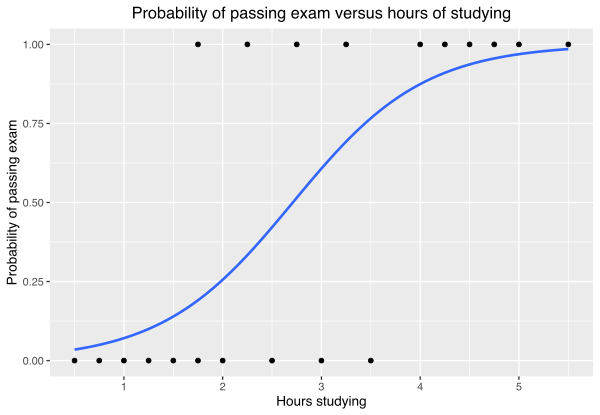
\includegraphics[scale=0.4]{wikiPassingExams.png}
\centering
\caption{Logistic Function of Passing Exam Based on Hours Studying}
\label{fig:wikilogfunction}
\end{figure}

\subsection{Decision Tree versus Logistic Regression Classification of Iris Data}

With the current logistic regression model now used to categorize the Iris dataset and with the Iris dataset split into \(\frac{1}{3}\) test data and \(\frac{2}{3}\) training data, a new linear equation was created. The calculated coefficients of the linear model were were $\beta_0 = 9.25$ (vertical intercept), $\beta_1 = -0.44$, $\beta_2 = -0.79$, $\beta_3 = -2.25$, and $\beta_4 = -0.98$.

When comparing the results of the logistic regression model with results from the secondary Decision Tree model, the accuracy of the test data and the r2 score were much greater in the logistic regression model. 

\begin{table}[h!]
\centering
\begin{tabular}{ c | c c c }
Model & Train Accuracy & Test Accuracy & r2 Score \\ 
\hline
Logistic Regression	& 0.98	& 0.94	& 0.905 \\
Decision Tree & 	1.00	& 0.92	& 0.874
\end{tabular}
\caption{Model Performance Comparison}
\label{table:model-comparison-table}
\end{table}

As the current logistic regression model included the default parameter of \lstinline{penalty='l2'}, a different iteration of the model with \lstinline{penalty=None} was also compared with the results from the Decision Tree model. These three models (Decision Tree, logistic regression with penalty, and logistic regression without penalty) were all run 1000 times each. 

\begin{table}[h!]
\centering
\begin{tabular}{ c | c c c }
    Description & Train Data Accuracy & Test Data Accuracy & r2 Score \\
\hline
count   &            1000.0   &      1000.000 &  1000.000\\
mean    &               1.0   &         0.930 &     0.889\\
std     &               0.0   &         0.015 &     0.024\\
min     &               1.0   &         0.920 &     0.873\\
25\%    &                1.0  &          0.920 &     0.873\\
50\%    &                1.0  &          0.920 &     0.873\\
75\%    &                1.0  &          0.940 &     0.905\\
max     &               1.0   &         0.960 &     0.936\\
\end{tabular}
\caption{Statistics for Decision Tree utilizing Gini Impurity Criterion}
\label{table:dtGI}
\end{table}

\begin{table}[h!]
\centering
\begin{tabular}{ c | c c c }
    Description & Train Data Accuracy & Test Data Accuracy & r2 Score \\
\hline
count       &       1000.00    &         1000.00&  1000.000 \\
mean        &          0.98    &            0.94&     0.905 \\
std         &          0.00    &            0.00&     0.000 \\
min         &          0.98    &            0.94 &    0.905 \\
25\%        &           0.98   &             0.94 &    0.905 \\
50\%        &           0.98   &             0.94 &    0.905 \\
75\%        &           0.98   &             0.94 &    0.905 \\
max         &          0.98    &            0.94  &   0.905 \\
\end{tabular}
\caption{Statistics for Logistic Regression with L2 Penalty}
\label{table:logRegL2}
\end{table}

\begin{table}[h!]
\centering
\begin{tabular}{ c | c c c }
    Description & Train Data Accuracy & Test Data Accuracy & r2 Score \\
\hline
count      &         1000.0     &        1000.00 & 1000.000\\
mean       &            1.0      &          0.96 &    0.936\\
std        &            0.0      &          0.00 &    0.000\\
min        &            1.0      &          0.96 &    0.936\\
25\%       &             1.0     &           0.96 &    0.936\\
50\%       &             1.0     &           0.96 &    0.936\\
75\%        &            1.0     &           0.96 &    0.936\\
max        &            1.0      &          0.96  &   0.936\\
\end{tabular}
\caption{Statistics for Logistic Regression without Penalty}
\label{table:logRegL2}
\end{table}

As the accuracy converges for each model, these methods can be more effectively compared. From these tables, it can be inferred that the logistic regression models are better predictors of the iris dataset. The decision tree model had an average accuracy of .93 when applied to the test datasets whereas the logistic models had accuracies of .94 and .96, with penalty and without respectively. As seen in the past, the decision tree's training data accuracy was 1.0 and the test data accuracy was much lower at .93 which indicates overfitting to the training dataset. 

Comparing the logistic models specifically, the model without implementing any penalty functions seems to perform better with a mean accuracy of .96. The accuracy for the model with penalty was .94. The r2 scores have a similar trend where the model without penalty had a mean r2 score of .936 and the model with penalty had a score of .905. For the iris dataset, the logistic model without penalty is the best choice.

\subsection{New Classifications Using Logistic Regression}

When using the \lstinline{predict_proba} function to create a ranking of the results of the logistic regression model, the output was compared to the original Iris dataset to see how the model probabilities compare to the actual Iris flower classification. A truncated version of this dataframe with randomly selected results is shown below:

\begin{table}[h!]
\centering
\begin{tabular}{ c | c c c }
Sample & Prob of setosa (0) &	Prob of versicolor (1) & Prob of virginica (2) \\ 
\hline
129	& 0.000	& 0.189	& 0.811 \\
42	& 0.988	& 0.012	& 0.000 \\
79	& 0.106	& 0.885	& 0.009 \\
30	& 0.965	& 0.035	& 0.000 \\
133	& 0.001	& 0.440	& 0.559
\end{tabular}
\caption{Results Sample}
\label{table:model-comparison-table}
\end{table}

The probabilities of setosa, versicolor, and virginica correspond to how likely the Iris flower is actually classified as the class. The higher the probability (closer to 1), the more likely the model categorizes the flower as being that class. For example, the first row shows that the flower has a 0 probability of being classified as setosa, 0.189 as versicolor, and 0.811 as virginica. Therefore it is most likely that the flower is actually Iris virginica. When referring to the original Iris dataset, one can confirm that this is indeed correct, the flower was an Iris virginica. 

The rankings and comparisons with the original Iris dataset seem to further confirm the accuracy of the model. This holds true even in the case of the fifth row, where the probabilities of versicolor and virginica are both fairly close together and near 0.5. The model shows that the probability of the flower being virginica is still higher than versicolor and the actual flower is classified as an Iris virginica. 

Given the two new data records (measurements of two new flowers), the probabilities of each flower class can be calculated. This table is shown below: 
    
\begin{table}[h!]
\centering
\begin{tabular}{ c | c c }
 & Enrty 1 &	Entry 2 \\ 
\hline
sepal length (cm)	& 5.800000	& 6.000000 \\
sepal width (cm)	& 2.800000	& 2.200000 \\
petal length (cm)	& 5.100000	& 4.000000 \\
petal width (cm)	& 2.400000	& 1.000000 \\
Prediction	& 2.000000	& 1.000000 \\
Prob of setosa (0)	& 0.000166	& 0.012343 \\
Prob of versicolor (1)	& 0.076790	& 0.966225 \\
Prob of virginica (2)	& 0.923044	& 0.021431
\end{tabular}
\caption{New Entry Classification}
\label{table:new-entry-table}
\end{table}

It can be seen, using the Prediction row, that the first record is predicted to be an Iris virginica (with a probability of 0.923) and the second record is predicted to be an Iris versicolor (with a probability of 0.966).

\section{Discussion}



\begin{thebibliography}{00}
\bibitem{b1}
“What is Logistic regression? | IBM.” https://www.ibm.com/topics/logistic-regression (accessed Sep. 23, 2023).
\bibitem{b2}
“Python Machine Learning - Logistic Regression.” https://www.w3schools.com/python/python-ml-logistic-regression.asp (accessed Sep. 23, 2023).
\bibitem{b3}
“Logistic regression,” Wikipedia. Aug. 31, 2023. Accessed: Sep. 22, 2023. [Online].
\bibitem{b4}
“How is L2 (ridge) penalty calculated in sklearn LogisticRegression function? | Saturn Cloud Blog,” Jul. 10, 2023. https://saturncloud.io/blog/how-is-l2-ridge-penalty-calculated-in-sklearn-logisticregression-function/ (accessed Sep. 23, 2023).

\end{thebibliography}

\end{document}